% *******************************************************************************
% * Copyright (c) 2007 by Elexis
% * All rights reserved. This document and the accompanying materials
% * are made available under the terms of the Eclipse Public License v1.0
% * which accompanies this distribution, and is available at
% * http://www.eclipse.org/legal/epl-v10.html
% *
% * Contributors:
% *    G. Weirich - initial implementation
% *
% *  $Id: patneu.tex 4903 2009-01-03 11:44:22Z rgw_ch $
% *******************************************************************************
% !Mode:: "TeX:UTF-8" (encoding info for WinEdt)

Démarrez Elexis en double-cliquant sur l'icône du programme. Après un bref
moment, une fenêtre apparaît comme dans la Figure  \ref{fig:startbild} (à condition que vous utilisez la base de données de démonstration, sinon les fenêtres apparaîtront vide) \footnote{La majorité des figures de cette visite guidée proviennent de Windows XP. L'apparence va différer légèrement sous d'autres systèmes d'exploitation}.
 \begin{figure}[ht]
    \center
	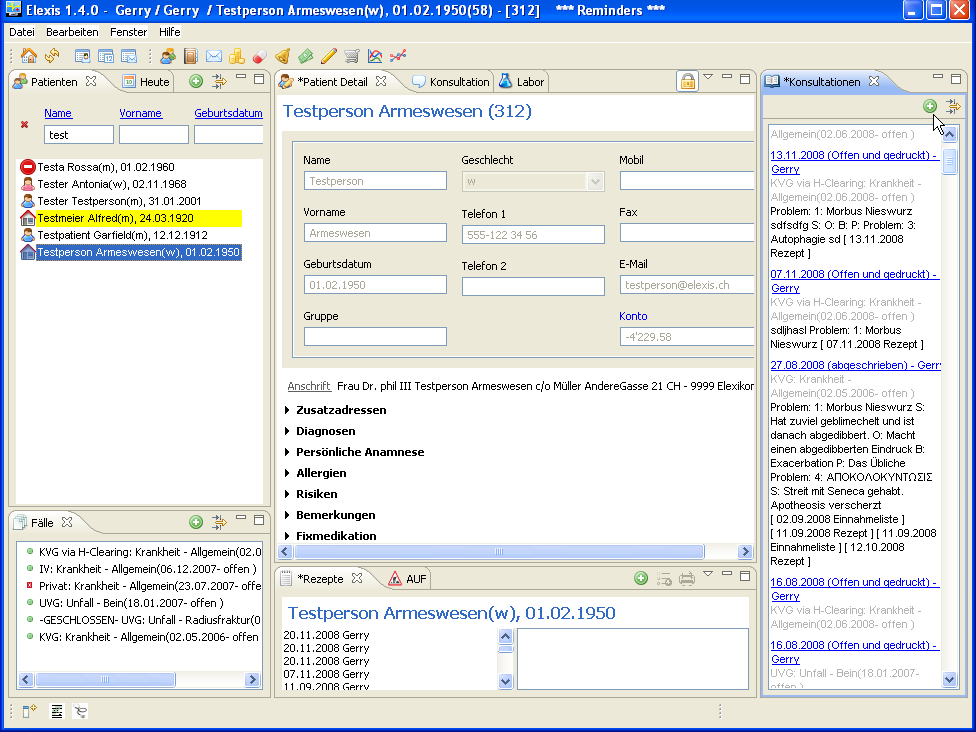
\includegraphics[width=0.9\textwidth]{images/einf0}
    %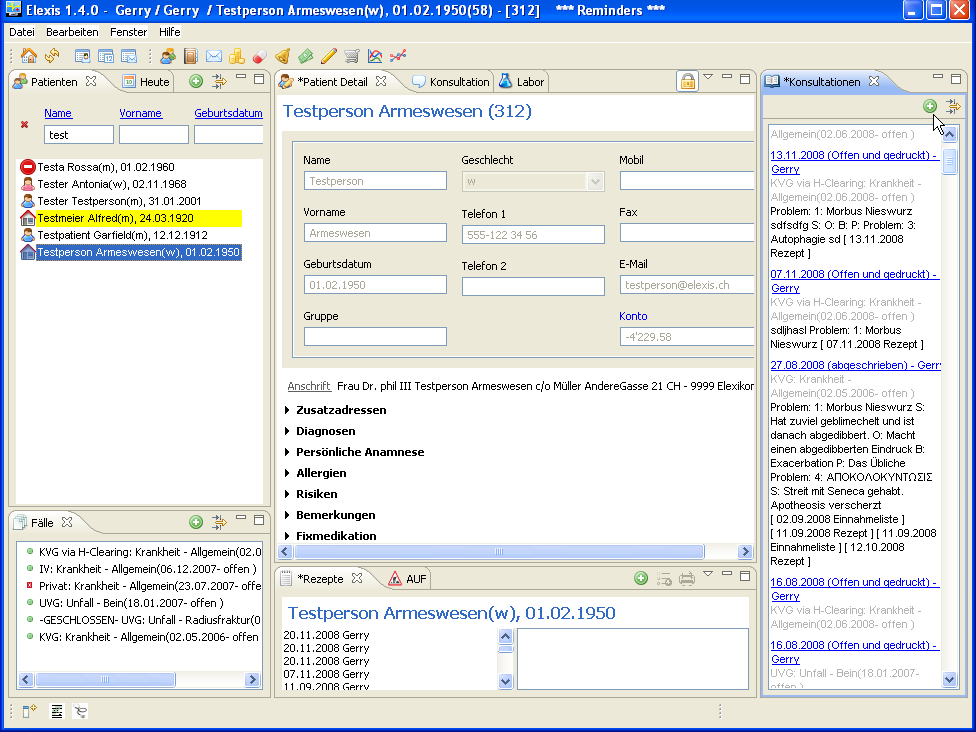
\includegraphics{images/einf0}
	\caption{Elexis Startbildschirm}
	\label{fig:startbild}
\end{figure}
\section{Saisir données des patients}
\begin{wrapfigure}{r}{8cm}
	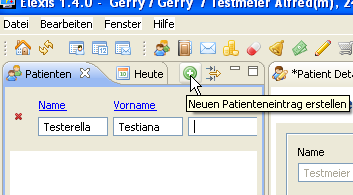
\includegraphics[width=6.5cm]{images/einf1}
	\caption{Patientennamen eingeben}\label{fig:patname}
\end{wrapfigure}
Activez en un clic l'affichage 'patients' et écrivez dans les champs de saisie Nom et Prénom de la nouvelle patiente.
Si la saisie de la patiente a déjà été faite, son nom apparaît. Dans notre cas, l'absence de patiente avec ce nom se montre par le manque d'une affiche.(cf Fig. \ref{fig:patname})\footnote{Pour vider les champs de saisie pour voir de nouveau tout les patients cliquez simplement sur la croix rouge qui se trouve à gauche du champ de saisie}.

\index{patient!nouveau}
Cliquez ensuite sur le bouton vert avec la croix blanche en haut à droite pour introduire les
données d'une nouvelle patiente.
Il apparaît une boîte de dialogue (Fig. \ref{fig:patdata}), où vous pouvez saisir les données dans les champs réservés.\\
\bigskip

\begin{figure}[ht]
	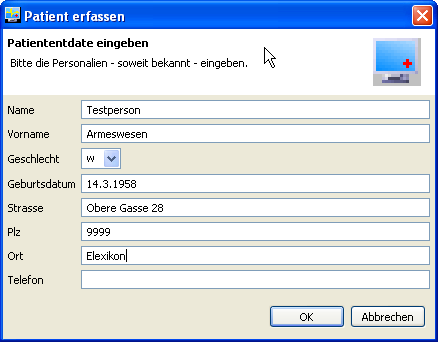
\includegraphics{images/einf2}
	\caption{Patientendaten ergänzen}
	\label{fig:patdata}
\end{figure}
Vous n'avez pas besoin d'introduire les données ici demandées de façon complète, mais simplement dans la mesure où ces donnés vous sont connus pour le moment. Vous n'êtes donc pas contraint pendant le service de la garde de d'abord introduire la totalité des données avant de pouvoir commencer un traitement.
Saisissez par exemple seulement le nom et la date de naissance et laissez introduire le reste plus tard par votre assistante médicale. Pour Elexis un nouveau patient est connu à partir du moment où vous cliquez sur 'OK' - peu importe combien de données du patient ont déjà été introduits à ce moment.


\section{Saisir données du cas}
S'il s'agit d'une nouvelle patiente, vous devez d'abord créer un  \glqq cas\grqq{} auquel la consultation peut être attribuée.
\index{Saisir!cas}

\begin{figure}[htbp]
     \begin{minipage}{0.4\textwidth}
      \centering
       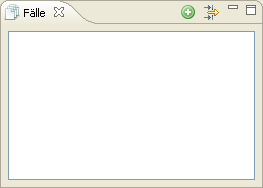
\includegraphics[width=0.8\textwidth]{images/einf3}
       \caption{Fälle-Ansicht}
       	\label{fig:faelle1}
     \end{minipage}\hfill
     \begin{minipage}{0.6\textwidth}
      \centering
       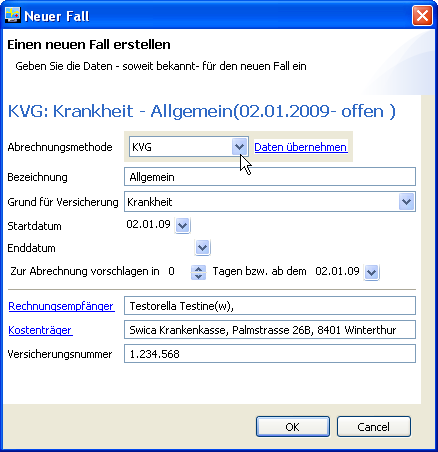
\includegraphics[width=1.0\textwidth]{images/einf4}
       \caption{Fall-Detail}
       \label{fig:falldetail}
     \end{minipage}
   \end{figure}


Un cas rassemble toutes les consultations qui sont saisies avec un système de facturation commun. (voir \ref{settings:abrechnungssystem} à la page \pageref{settings:abrechnungssystem}).
Cliquez donc dans l'affichage \glqq cas\grqq{}(Fig. \ref{fig:faelle1}) sur le bouton vert avec la croix blanche '= Nouveau'.

Cela ouvrira une boîte de dialogue pour inscrire les données dans la mesure où elles vous sont connues (Fig. \ref{fig:falldetail})

Au plus tard lors de la facturation les informations nécessaires (débiteur, répondant des coûts et numéro d'assurance respectivement numéro de cas) doivent toutefois être introduites. Après avoir cliqué sur OK, vous avez créé un nouveau 'cas'. Bien évidemment,lors des consultations suivantes on peut s'épargner cette étape. \\

\bigskip

Ensuite nous créons une nouvelle consultation en cliquant sur l'onglet " Consultation " et en choisissant de nouveau le fameux bouton vert à la croix blanche (Fig. \ref{fig:neuekons}.

\index{Consultation!nouvelle}
\begin{figure}[ht]
	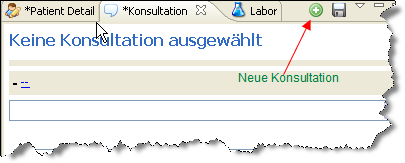
\includegraphics{images/einf5}
	\caption{Neue Konsultation}
	\label{fig:neuekons}
\end{figure}
\pagebreak[2]

Ensuite, on peut commencer introduire des informations médicales dans le dossier du patient (Fig. \ref{fig:KG}).

\section{Gérer le dossier médical}
\begin{figure}
    \begin{center}
	   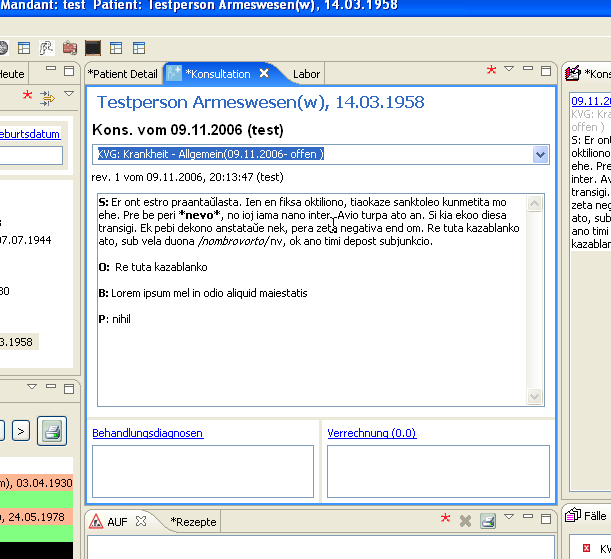
\includegraphics[width=0.7\textwidth]{images/einf6}
    	\caption{KG-Eintrag}
	   \label{fig:KG}
    \end{center}
\end{figure}
Les notes introduites dans le dossier médical peuvent contenir des simples mise en forme du texte. Des blocs de texte peuvent être définis librement et peuvent être activés par une touche de raccourci clavier ('shortcut') configurable.
La comptabilisation se fera alors soit par un macro attribué à une touche du clavier soit par la souris. Après avoir introduit les informations dans le dossier médical (ou même avant ou pendant) vous pouvez cliquer sur \glqq saisie prestation\grqq{} pour ouvrir la fenêtre de saisie des prestations.(Fig. \ref{fig:Verrechnung}. En analogie vous pouvez cliquer sur \glqq diagnostics\grqq{} pour ouvrir la vue des diagnostics.

\begin{figure}[ht]
	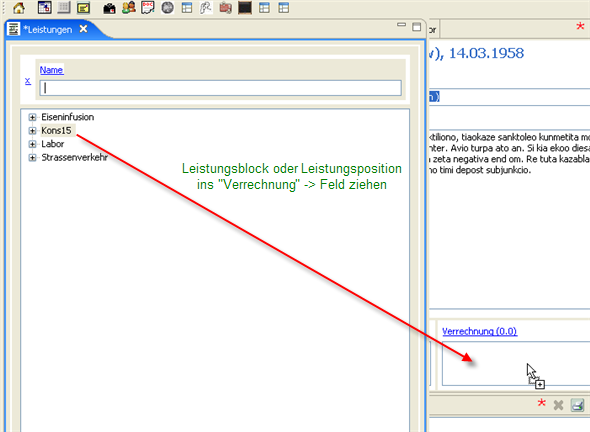
\includegraphics[width=6cm]{images/einf7}
	\caption{Verrechnungs-Fenster}
	\label{fig:Verrechnung}
\end{figure}
Cette fenêtre contient toutes les systèmes de prestations codifiés prévues dans le logiciel ainsi qu'une page avec des blocs de prestation prédéfinis par vous même.
\index{Saisie!prestations}\index{saisie}
Vous pouvez glisser (drag and drop) soit l'ensemble d'un bloc ou des prestations isolées d'un bloc ou d'une autre fenêtre de prestation (Tarmed etc.) dans le champ de
 \glqq saisie prestation \grqq{}.

De la même façon on peut associer des diagnostics à une consultation et aussi dans ce cas, on a le choix de tous les différents systèmes de codification des diagnostics intégrés dans le logiciel (tout ceci adaptable et extensible).
\index{consultation!diagnostic}

\clearpage
